% Options for packages loaded elsewhere
\PassOptionsToPackage{unicode}{hyperref}
\PassOptionsToPackage{hyphens}{url}
%
\documentclass[
  10pt,
  letterpaper,
  DIV=11,
  numbers=noendperiod,
  twoside]{scrartcl}

\usepackage{amsmath,amssymb}
\usepackage{setspace}
\usepackage{iftex}
\ifPDFTeX
  \usepackage[T1]{fontenc}
  \usepackage[utf8]{inputenc}
  \usepackage{textcomp} % provide euro and other symbols
\else % if luatex or xetex
  \usepackage{unicode-math}
  \defaultfontfeatures{Scale=MatchLowercase}
  \defaultfontfeatures[\rmfamily]{Ligatures=TeX,Scale=1}
\fi
\usepackage{lmodern}
\ifPDFTeX\else  
    % xetex/luatex font selection
    \setmainfont[ItalicFont=EB Garamond Italic,BoldFont=EB Garamond
Bold]{EB Garamond Math}
    \setsansfont[]{Europa-Bold}
  \setmathfont[]{Garamond-Math}
\fi
% Use upquote if available, for straight quotes in verbatim environments
\IfFileExists{upquote.sty}{\usepackage{upquote}}{}
\IfFileExists{microtype.sty}{% use microtype if available
  \usepackage[]{microtype}
  \UseMicrotypeSet[protrusion]{basicmath} % disable protrusion for tt fonts
}{}
\usepackage{xcolor}
\usepackage[left=1in, right=1in, top=0.8in, bottom=0.8in,
paperheight=9.5in, paperwidth=6.5in, includemp=TRUE, marginparwidth=0in,
marginparsep=0in]{geometry}
\setlength{\emergencystretch}{3em} % prevent overfull lines
\setcounter{secnumdepth}{3}
% Make \paragraph and \subparagraph free-standing
\makeatletter
\ifx\paragraph\undefined\else
  \let\oldparagraph\paragraph
  \renewcommand{\paragraph}{
    \@ifstar
      \xxxParagraphStar
      \xxxParagraphNoStar
  }
  \newcommand{\xxxParagraphStar}[1]{\oldparagraph*{#1}\mbox{}}
  \newcommand{\xxxParagraphNoStar}[1]{\oldparagraph{#1}\mbox{}}
\fi
\ifx\subparagraph\undefined\else
  \let\oldsubparagraph\subparagraph
  \renewcommand{\subparagraph}{
    \@ifstar
      \xxxSubParagraphStar
      \xxxSubParagraphNoStar
  }
  \newcommand{\xxxSubParagraphStar}[1]{\oldsubparagraph*{#1}\mbox{}}
  \newcommand{\xxxSubParagraphNoStar}[1]{\oldsubparagraph{#1}\mbox{}}
\fi
\makeatother


\providecommand{\tightlist}{%
  \setlength{\itemsep}{0pt}\setlength{\parskip}{0pt}}\usepackage{longtable,booktabs,array}
\usepackage{calc} % for calculating minipage widths
% Correct order of tables after \paragraph or \subparagraph
\usepackage{etoolbox}
\makeatletter
\patchcmd\longtable{\par}{\if@noskipsec\mbox{}\fi\par}{}{}
\makeatother
% Allow footnotes in longtable head/foot
\IfFileExists{footnotehyper.sty}{\usepackage{footnotehyper}}{\usepackage{footnote}}
\makesavenoteenv{longtable}
\usepackage{graphicx}
\makeatletter
\newsavebox\pandoc@box
\newcommand*\pandocbounded[1]{% scales image to fit in text height/width
  \sbox\pandoc@box{#1}%
  \Gscale@div\@tempa{\textheight}{\dimexpr\ht\pandoc@box+\dp\pandoc@box\relax}%
  \Gscale@div\@tempb{\linewidth}{\wd\pandoc@box}%
  \ifdim\@tempb\p@<\@tempa\p@\let\@tempa\@tempb\fi% select the smaller of both
  \ifdim\@tempa\p@<\p@\scalebox{\@tempa}{\usebox\pandoc@box}%
  \else\usebox{\pandoc@box}%
  \fi%
}
% Set default figure placement to htbp
\def\fps@figure{htbp}
\makeatother
% definitions for citeproc citations
\NewDocumentCommand\citeproctext{}{}
\NewDocumentCommand\citeproc{mm}{%
  \begingroup\def\citeproctext{#2}\cite{#1}\endgroup}
\makeatletter
 % allow citations to break across lines
 \let\@cite@ofmt\@firstofone
 % avoid brackets around text for \cite:
 \def\@biblabel#1{}
 \def\@cite#1#2{{#1\if@tempswa , #2\fi}}
\makeatother
\newlength{\cslhangindent}
\setlength{\cslhangindent}{1.5em}
\newlength{\csllabelwidth}
\setlength{\csllabelwidth}{3em}
\newenvironment{CSLReferences}[2] % #1 hanging-indent, #2 entry-spacing
 {\begin{list}{}{%
  \setlength{\itemindent}{0pt}
  \setlength{\leftmargin}{0pt}
  \setlength{\parsep}{0pt}
  % turn on hanging indent if param 1 is 1
  \ifodd #1
   \setlength{\leftmargin}{\cslhangindent}
   \setlength{\itemindent}{-1\cslhangindent}
  \fi
  % set entry spacing
  \setlength{\itemsep}{#2\baselineskip}}}
 {\end{list}}
\usepackage{calc}
\newcommand{\CSLBlock}[1]{\hfill\break\parbox[t]{\linewidth}{\strut\ignorespaces#1\strut}}
\newcommand{\CSLLeftMargin}[1]{\parbox[t]{\csllabelwidth}{\strut#1\strut}}
\newcommand{\CSLRightInline}[1]{\parbox[t]{\linewidth - \csllabelwidth}{\strut#1\strut}}
\newcommand{\CSLIndent}[1]{\hspace{\cslhangindent}#1}

\setlength\heavyrulewidth{0ex}
\setlength\lightrulewidth{0ex}
\usepackage[automark]{scrlayer-scrpage}
\clearpairofpagestyles
\cehead{
  Brian Weatherson
  }
\cohead{
  From Classical to Intuitionistic Probability
  }
\ohead{\bfseries \pagemark}
\cfoot{}
\makeatletter
\newcommand*\NoIndentAfterEnv[1]{%
  \AfterEndEnvironment{#1}{\par\@afterindentfalse\@afterheading}}
\makeatother
\NoIndentAfterEnv{itemize}
\NoIndentAfterEnv{enumerate}
\NoIndentAfterEnv{description}
\NoIndentAfterEnv{quote}
\NoIndentAfterEnv{equation}
\NoIndentAfterEnv{longtable}
\NoIndentAfterEnv{abstract}
\renewenvironment{abstract}
 {\vspace{-1.25cm}
 \quotation\small\noindent\rule{\linewidth}{.5pt}\par\smallskip
 \noindent }
 {\par\noindent\rule{\linewidth}{.5pt}\endquotation}
\KOMAoption{captions}{tableheading}
\makeatletter
\@ifpackageloaded{caption}{}{\usepackage{caption}}
\AtBeginDocument{%
\ifdefined\contentsname
  \renewcommand*\contentsname{Table of contents}
\else
  \newcommand\contentsname{Table of contents}
\fi
\ifdefined\listfigurename
  \renewcommand*\listfigurename{List of Figures}
\else
  \newcommand\listfigurename{List of Figures}
\fi
\ifdefined\listtablename
  \renewcommand*\listtablename{List of Tables}
\else
  \newcommand\listtablename{List of Tables}
\fi
\ifdefined\figurename
  \renewcommand*\figurename{Figure}
\else
  \newcommand\figurename{Figure}
\fi
\ifdefined\tablename
  \renewcommand*\tablename{Table}
\else
  \newcommand\tablename{Table}
\fi
}
\@ifpackageloaded{float}{}{\usepackage{float}}
\floatstyle{ruled}
\@ifundefined{c@chapter}{\newfloat{codelisting}{h}{lop}}{\newfloat{codelisting}{h}{lop}[chapter]}
\floatname{codelisting}{Listing}
\newcommand*\listoflistings{\listof{codelisting}{List of Listings}}
\makeatother
\makeatletter
\makeatother
\makeatletter
\@ifpackageloaded{caption}{}{\usepackage{caption}}
\@ifpackageloaded{subcaption}{}{\usepackage{subcaption}}
\makeatother
\makeatletter
\@ifpackageloaded{sidenotes}{}{\usepackage{sidenotes}}
\@ifpackageloaded{marginnote}{}{\usepackage{marginnote}}
\makeatother

\usepackage{bookmark}

\IfFileExists{xurl.sty}{\usepackage{xurl}}{} % add URL line breaks if available
\urlstyle{same} % disable monospaced font for URLs
\hypersetup{
  pdftitle={From Classical to Intuitionistic Probability},
  pdfauthor={Brian Weatherson},
  hidelinks,
  pdfcreator={LaTeX via pandoc}}


\title{From Classical to Intuitionistic Probability}
\author{Brian Weatherson}
\date{2001}

\begin{document}
\maketitle
\begin{abstract}
We generalize the Kolmogorov axioms for probability calculus to obtain
conditions defining, for any given logic, a class of probability
functions relative to that logic, coinciding with the standard
probability functions in the special case of classical logic but
allowing consideration of other classes of ``essentially Kolmogorovian''
probability functions relative to other logics. We take a broad view of
the Bayesian approach as dictating \emph{inter alia} that from the
perspective of a given logic, rational degrees of belief are those
representable by probability functions from the class appropriate to
that logic. Classical Bayesianism, which fixes the logic as classical
logic, is only one version of this general approach. Another, which we
call Intuitionistic Bayesianism, selects intuitionistic logic as the
preferred logic and the associated class of probability functions as the
right class of candidate representions of epistemic states (rational
allocations of degrees of belief). Various objections to classical
Bayesianism are, we argue, best met by passing to intuitionistic
Bayesianism -- in which the probability functions are taken relative to
intuitionistic logic -- rather than by adopting a radically
non-Kolmogorovian, e.g.~non-additive, conception of (or substitute for)
probability functions, in spite of the popularity of the latter response
amongst those who have raised these objections. The interest of
intuitionistic Bayesianism is further enhanced by the availability of a
Dutch Book argument justifying the selection of intuitionistic
probability functions as guides to rational betting behaviour when due
consideration is paid to the fact that bets are settled only when/if the
outcome betted on becomes known.
\end{abstract}


\setstretch{1.1}
\section{Introduction}\label{introduction}

It is a standard claim of modern Bayesian epistemology that reasonable
epistemic states should be representable by probability functions. There
have been a number of authors who have opposed this claim. For example,
it has been claimed that epistemic states should be representable by
Zadeh's fuzzy sets, Dempster and Shafer's evidence functions, Shackle's
potential surprise functions, Cohen's inductive probabilities or
Schmeidler's non-additive probabilities.\footnote{For more details, see
  Zadeh (\citeproc{ref-Zadeh1978}{1978}), Dempster
  (\citeproc{ref-Dempster1967}{1967}), Shafer
  (\citeproc{ref-Shafer1976}{1976}), Shackle
  (\citeproc{ref-Shackle1949}{1949}), Cohen
  (\citeproc{ref-Cohen1977}{1977}), Schmeidler
  (\citeproc{ref-Schmeidler1989}{1989}).} A major motivation of these
theorists has been that in cases where we have little or no evidence for
or against \emph{p}, it should be reasonable to have low degrees of
belief in each of \emph{p} and ¬\emph{p}, something apparently
incompatible with the Bayesian approach. There are two broad types of
response to this situation, the second of which shows the
incompatibility just mentioned is more apparent than real. The first of
these -- much in evidence in the work of the writers just cited -- is to
replace or radically reconstrue the notion of probability taken by that
approach to represent degrees of belief. The second -- to be defended
here -- seeks to maintain the core of standard probability theory but to
generalize the notion of a probability function to accommodate variation
in the background logic of the account; this allows us to respond to
such issues as the low degree of belief in a proposition and its
negation by simply weakening the background logic from classical to
intuitionistic logic. Thus if Bayesianism is construed as in our opening
sentence, one way to respond to the objections of the heterodox writers
listed above is to trade in \emph{classical} Bayesianism for
\emph{intuitionistic} Bayesianism. Since for many theorists at least the
motivation for their opposition to Bayesianism is grounded in either
verificationism or anti-realism, a move to a intuitionistic theory of
probability seems appropriate. Indeed, as Harman
(\citeproc{ref-Harman1983}{1983}) notes, the standard analysis of
degrees of belief as dispositions to bet leads naturally to a
intuitionistic theory of probability. We give a Dutch Book argument in
defence of constructive Bayesianism in Section 4 below.

The appropriate generalization of the notion of a probability function
makes explicit allowance for a sensitivity to the background logic. The
latter we identify with a consequence relation, such as, in particular,
the consequence relation \(\vdash_{CL}\) associated with classical logic
or the consequence relation \(\vdash_{IL}\) associated with
intuitionistic logic. To keep things general, we assume only that the
languages under discussion have two binary connectives:~∨~and ~∧. No
assumptions are made about how a consequence relation on such a language
treats compounds formed using these connectives, though of course in the
cases in which we are especially interested, \(\vdash_{CL}\) and
\(\vdash_{IL}\), such compounds have the expected logical properties. We
take the language of these two consequences relations to be the same,
assuming in particular that negation (¬) is present for both. Finally,
if \emph{A} belongs to the language of a consequence relation
\(\vdash\), then we say that \emph{A} is a \(\vdash\)-\emph{thesis} of
\(\vdash\) \emph{A} and that \emph{A} is a \(\vdash\)-\emph{antithesis}
if for all \emph{B} in that language \emph{A} \(\vdash\) \emph{B}. (Thus
the \(\vdash\)-theses and antitheses represent the logical truths and
logical falsehoods as seen from the perspective of \(\vdash\).) We are
now in a position to give the key definition.

If \(\vdash\) is a consequence relation, then a function \emph{Pr}
mapping the language of \(\vdash\) to the real interval {[}0,1{]} is a
\(\vdash\)\emph{-probability function} if and only if the following
conditions are satisfied:

\begin{description}
\tightlist
\item[(P0)]
\emph{Pr}(\emph{A}) = 0 if \emph{A} is a \(\vdash\)-antithesis.
\item[(P1)]
\emph{Pr}(\emph{A}) = 1 if \emph{A} is a \(\vdash\)-thesis
\item[(P2)]
If \emph{A}~\(\vdash\) \emph{B} then
\emph{Pr}(\emph{A})~\({\leq}\)~\emph{Pr}(\emph{B})
\item[(P3)]
\emph{Pr}(\emph{A})~+~\emph{Pr}(\emph{B}) =
\emph{Pr}(\emph{A}~∨~\emph{B})~+~\emph{Pr}(\emph{A}~~∧~\emph{B})
\end{description}

If \(\vdash\) is \(\vdash_{CL}\), then we call a \(\vdash\)-probability
function a \emph{classical probability function}; if \(\vdash\) is
\(\vdash_{IL}\) we call a \(\vdash\)-probability function an
\emph{intuitionistic} \emph{probability function}. The position
described above as constructive Bayesianism would replace classical
probability functions by intuitionistic probability functions as
candidate representations of reasonable epistemic states. Note that
classical probability functions in this sense are exactly those obeying
the standard probability calculus axioms. In paricular, the familiar
negation axiom dictating that \emph{Pr}( ¬\emph{A}) = 1 --
\emph{Pr}(\emph{A}) emerges as a by-product of the interaction between
the general (i.e., logic-independent) condition (P3) and, via (P0) and
(P1), the logic-specific facts that \emph{A}~~∧~¬\emph{A} is a
\(\vdash_{CL}\)-antithesis and \emph{A}~∨~¬\emph{A} is a
\(\vdash_{CL}\)-thesis for any \emph{A}.

Although it is these two kinds -- intuitionistic and classical -- of
probability functions we shall be dealing with specifically in what
follows, we emphasize the generality of the above definition of a
\(\vdash\)-probability function, and invite the reader to consider what
effect further varying the choice of \(\vdash\) has on the behaviour of
such functions. Our attention will be on the comparative merits of
\(\vdash_{CL}\) and \(\vdash_{IL}\) in this regard. (It may have
occurred to the reader in connection with (P3) above that we might
naturally have considered a generalized version of (P3) for `countable
additivity'. Whether such a condition ought be adopted will turn on some
rather difficult questions concerning the use of infinities in
constructive reasoning; let us leave it as a question for further
research. We have stated (P3) in its finitary form so as not to require
that intuitionistic probability functions satisfy the more contentious
general condition.)

In the following section we shall review some of the motivations for
intuitionistic Bayesianism. The arguments are rather piecemeal; they are
designed to show that given the philosophical commitments various
writers in the field have expressed they would be better off taking this
route, i.e., focussing on the class of intuitionistic probability
functions, than -- as many of them have suggested --abandoning
Bayesianism in our broad sense. In particular, we shall urge that moves
in the latter direction which involve abandoning (what we shall call)
the Principle of Addition are seriously undermotivated.

One aspect of the Bayesian perspective which we have not considered
concerns the dynamics rather than the statics of epistemic states: in
particular the idea that changes in such states are governed for
rational agents by the principle of conditionalizing on new information.
This requires that we have a dyadic functor available for expressing
conditional probabilities. Accordingly, where \emph{Pr} is for some
consequence relation \(\vdash\) a \(\vdash\)-probability function, we
favour the standard account and take the associated conditional
\(\vdash\)-probability function \emph{Pr}( , ) to be given by
\emph{Pr}(\emph{A},\emph{B}) =
\emph{Pr}(\emph{A}~~∧~\emph{B})/\emph{Pr}(\emph{B}) when
\emph{Pr}(\emph{B}) \({\neq}\) 0, with \emph{Pr}(\emph{A},\emph{B})
undefined when \emph{Pr}(\emph{B}) = 0. The intention, of course, is
that \emph{Pr}(\emph{A},\emph{B}) represents the conditional probability
of \emph{A} given \emph{B}. We defer further consideration of
conditional probability until the Appendix.

\section{Motivating Intuitionistic
Bayesianism}\label{motivating-intuitionistic-bayesianism}

There are four main reasons for grounding preferring intuitionistic over
classical probability functions as representing the range of reasonable
epistemic states. These are: (1) a commitment to verificationism, (2) a
commitment to anti-realism, (3) preservation of the principle of
Addition, and (4) avoidance of direct arguments for the orthodox
approach. Now some of these will be viewed by some people as bad reasons
for adopting the given position, a reaction with which it is not hard to
sympathise. In particular, the verificationist and anti-realist elements
of the theory might well be viewed as negatives. These arguments are
principally directed at showing that by their own lights, various
opponents of classical Bayesianism would do better to adopt the
intuitionistic Bayesian position than some still more heterodox
non-Bayesian account.

\textbf{2.1} A standard objection to classical Bayesianism is that it
has no way of representing complete uncertainty. Because of the failures
of Laplace's principle of indifference, it can't be said that
uncertainty about \emph{p} is best represented by assigning credence 1/2
to \emph{p}. Heterodox approaches usually allow the assignment of
credence 0 to both \emph{p} and ¬\emph{p} when an agent has no evidence
at all as to whether or not \emph{p} is true. Because these approaches
generally require an agent to assign credence 1 to classical
tautologies, including \emph{p}~∨~¬\emph{p}, these theories must give up
the following principle of \textbf{Addition}.

\begin{quote}
\textbf{Addition}\\
For incompatible \emph{A}, \emph{B}:
\emph{Bel}(\emph{A}~∨~\emph{B})~=~\emph{Bel}(\emph{A})~+~\emph{Bel}(\emph{B}).
\end{quote}

``\emph{Bel}(\emph{A})'' is here used to mean the degree of belief the
agent has in \emph{A}, and ``incompatible'' to apply to \emph{A} and
\emph{B} in which for some favoured consequence relation \(\vdash\), the
conjunction of \emph{A} with \emph{B} is a \(\vdash\)-antithesis. Such
conditions as Addition are of course taken not as descriptive theories
about all agents, since irrational agents would serve as
counterexamples. Rather, they are proposed coherence constraints on all
rational agents.

The Principle of Addition is stated in terms of degrees of belief, or
credences. Where no ambiguity results we also use the same term to refer
to the corresponding principle applied to \(\vdash\)-probability
functions, with incompatibility understood in terms of \(\vdash\) (as
just explained). Now in some writings (particularly Shafer's) the reason
suggested for giving up \emph{Addition} is openly verificationist.
Shafer says that when an agent has no evidence for \emph{p}, they should
assign degree of belief 0 to \emph{p}. Degrees of belief, under this
approach, must be proportional to evidence.\footnote{This assumption was
  shared by many of the participants in the symposium on probability in
  legal reasoning, reported in the Boston University Law Review 66
  (1986).} In recent philosophical literature, this kind of
verificationism is often accompanied by an insistence that validity of
arguments be judged by the lights of \(\vdash_{IL}\) rather than
\(\vdash_{CL}\).

A similar line of thought is to be found in Harman
(\citeproc{ref-Harman1983}{1983}). He notes that when we don't
distinguish between the truth conditions for a sentence and its
assertibility conditions, the appropriate logic is intuitionistic. And
when we're considering gambles, something like this is correct. When
betting on \emph{p} we don't, in general, care if \emph{p} is true as
opposed to whether it will be discovered that \emph{p} is true. A
\emph{p}-bet, where \emph{p} asserts the occurrence of some event for
instance, becomes a winning bet, not when that event occurs, but when
\emph{p} becomes assertible. So perhaps not just verificationists like
Shafer, but all those who analyse degrees of belief as propensity to bet
should adopt constructivist approaches to probability.

To see the point Harman is making, consider this example. We are invited
to quote for \emph{p}-bets and ¬\emph{p}-bets, where \emph{p} is
\emph{O. J. Simpson murdered his wife}. If we are to take the
Californian legal system literally, the probability of that given the
evidence is strictly between one-half and one. To avoid one objection,
these bets don't just pay \$1 if the bettor guesses correctly. Rather
they pay \$1 invested at market rates of interest at the time the bet is
placed. The idea is that if we pay \emph{x} cents for the bet now, when
it is discovered that we have bet correctly we will receive a sum of
money that is worth exactly as much as \$1 now. Still, we claim, it
might be worthwhile to quote less than 50 cents for each of the bets.
Even if we will receive \$1 worth of reward if we wager correctly, there
is every possibility that we'll never find out. So it might be that
placing a bet would be a losing play either way. To allow for this, the
sum of our quotes for the \emph{p}-bet and the ¬\emph{p}-bet may be less
than \$1. As Harman points out, to reply by wielding a Dutch Book
argument purporting to show that this betting practice is incoherent
would be blatantly question-begging. That argument simply assumes that
\emph{p}~∨~¬\emph{p} is a logical truth, which is presumably part of
what's at issue. (In our terminology, this disjunction has the status of
a \(\vdash_{CL}\)-thesis which is not a \(\vdash_{IL}\)-thesis.)

Harman's point is not to argue for a intuitionistic approach to
probability. Rather, he is arguing against using probabilistic semantics
for propositional logic. Such an approach he claims would be bound to
lead to intuitionistic logic for the reasons given above. He thinks
that, since this would be an error, the move to probabilistic semantics
is simply misguided. Whatever we think of this conclusion, we can press
into service his arguments for intuitionistic Bayesianism.

\textbf{2.2} The second argument for this approach turns on the
anti-realism of some heterodox theorists. So George Shackle, for
example, argues that if we are anti-realists about the future, we will
assign positive probability to no future-directed proposition. The
following summary is from a sympathetic interpreter of Shackle's
writing.

\begin{quote}
{[}T{]}here is every reason to refuse additivity: {[}it{]} implies that
the certainty that would be assigned to the set of possibilities should
be `distributed' between different events. Now this set of events is
undetermined as the future -- that exists only in imagination -- is.
(\citeproc{ref-Ponsonnet1996}{Ponsonnet 1996, 171})
\end{quote}

Shackle's anti-realism is motivated by what most theorists would regard
as a philosophical howler: he regards realism about the future as
incompatible with human freedom, and holds that human beings are free.
The second premise here seems harmless enough, but the first is
notoriously difficult to motivate. Nevertheless, there are some better
arguments than this for anti-realism about the future. If we adopt
these, it isn't clear why we should `assign certainty' to the set of
possibilities.

Shackle is here assuming that for any proposition \emph{p}, even a
proposition about the future, \emph{p}~∨~¬\emph{p} is now true, although
neither disjunct is true. Given his interests it seems better to follow
Dummett here and say that if we are anti-realists about a subject then
for propositions \emph{p} about that subject, \emph{p}~∨~¬\emph{p} fails
to be true. Hence we have no need to `assign certainty to the set of
possibilities'. Or perhaps more accurately, assigning certainty to the
set of possibilities does not mean assigning probability 1 to
\emph{p}~∨~¬\emph{p}; in particular, condition (P1) on
\(\vdash\)-probability functions does not require this when we choose
\(\vdash\) as \(\vdash_{IL}\).

\textbf{2.3} The third motivation for adopting an intuitionistic
approach to probability is that it allows us to retain the Kolmogorov
axioms for probability, in particular the Principle of Addition. This
principle has, to my mind at least, some intuitive motivation. And the
counterexamples levelled against it by heterodox theorists seem rather
weak from the intuitionistic Bayesian perspective. For they all are
cases where we might feel it appropriate to assign a low probability to
a proposition and its negation\footnote{Again the discussion in
  (\citeproc{ref-Shafer1976}{Shafer 1976} ch.~2) is the most obvious
  example of this, but similar examples abound in the literature.}.
Hence if we are committed to saying \emph{Pr}(\emph{A}~∨~¬\emph{A})~=~1
for all \emph{A}, we must give up the Principle of Addition. But the
intuitionistic Bayesian simply denies that in these cases
\emph{Pr}(\emph{A}~∨~¬\emph{A})~=~1, so no counterexample to Addition
arises. This denial is compatible with condition (P1) on \emph{Pr}'s
being a \(\vdash_{IL}\)-probability function since, as already noted,
\emph{A}~∨~¬\emph{A} is not in general a
\(\vdash_{IL}\)\emph{-}thesis\emph{.}

\textbf{2.4} The final argument for taking an intuitionistic approach is
that it provides a justification for rejecting the positive arguments
for classical Bayesianism. These provide a justification for requiring
coherent degrees of belief to be representable by the classical
probability calculus. There are a dizzying variety of such arguments
which link probabilistic epistemology to decision theory, including: the
traditional Dutch Book arguments found in Ramsey
(\citeproc{ref-RamseyTruthProb}{1926}), Teller
(\citeproc{ref-Teller1973}{1973}) and Lewis
(\citeproc{ref-Lewis1999b}{1999}); de-pragmatized Dutch Book arguments
which rely on consistency of valuations, rather than avoiding actual
losses, as in Howson and Urbach (\citeproc{ref-HowsonUrbach1989}{1989}),
Christensen (\citeproc{ref-Christensen1996}{1996}) and Hellman
(\citeproc{ref-Hellman1997}{1997}); and arguments from the plausibility
of decision theoretic constraints to constraints on partial beliefs, as
in Savage (\citeproc{ref-Savage1954}{1954}), Maher
(\citeproc{ref-Maher1993}{1993}) and Kaplan
(\citeproc{ref-Kaplan1996}{1996}). As well as these, there are arguments
for classical Bayesianism which do not rely on decision theory in any
way, but which flow either directly from the definitions of degrees of
belief, or from broader epistemological considerations. A summary of
traditional arguments of this kind is in Paris
(\citeproc{ref-Paris1994}{1994}). Joyce (\citeproc{ref-Joyce1998}{1998})
provides an interesting modern variation on this theme.

All such arguments assume classical -- rather than, say, intuitionistic
-- reasoning is appropriate. The intuitionist has a simple and
principled reason for rejecting those arguments. The theorist who
endorses \(\vdash_{CL}\) when considering questions of inference,
presumably lacks any such simple reason. And they need one, unless they
think it appropriate to endorse one position knowing there is an
unrefuted argument for an incompatible viewpoint.

We are not insisting that non-Bayesians will be unable to refute these
arguments while holding on to \(\vdash_{CL}\). We are merely suggesting
that the task will be Herculean. A start on this project is made by
Shafer (\citeproc{ref-Shafer1981}{1981}), which suggests some reasons
for breaking the link between probabilistic epistemology and decision
theory. Even if these responses are successful, such a response is
completely ineffective against arguments which do not exploit such a
link. As we think these are the strongest arguments for classical
Bayesianism, non-Baeyesians have much work left to do. And it is
possible that this task cannot be completed. That is, it is possible
that the only questionable step in some of these arguments for classical
Bayesianism is their use of non-constructive reasoning. If this is so
only theorists who give up \(\vdash_{CL}\) can respond to such
arguments.

In sum, non-Bayesians need to be able to respond to the wide variety of
arguments for Bayesianism. Non-Bayesians who hold on to \(\vdash_{CL}\)
must do so without questioning the implicit logical assumptions of such
arguments. Given this restriction, producing these responses will be a
slow, time-consuming task, the responses will in all likelihood be
piecemeal, providing little sense of the underlying flaw of the
arguments, and for some arguments it is possible that no effective
response can be made. Intuitionistic Bayesians have a quick, systematic
and, we think, effective response to all these arguments.

\section{More on Intuitionistic Probability
Functions}\label{more-on-intuitionistic-probability-functions}

Having explained the motivation for intuitionistic Bayesianism, let us
turn our attention in greater detail to its main source of novelty: the
intuitionistic probability functions. We concentrate on logical matters
here, in the following section justifying the singling out of this class
of probability functions by showing that an epistemic state represented
by \emph{Bel} is invulnerable to a kind of Dutch Book if and only if
\emph{Bel} is an intuitionistic probability function.

For the case of specifically \emph{classical} probability functions, the
conditions (P0)--(P4) of Section 1 involve substantial redundancy. For
example, we could replace (P2) and (P3) by -- what would in isolation be
weaker conditions -- (P2′) and (P3′).

\begin{description}
\tightlist
\item[(P2\(^\prime\))]
If \emph{A} \(\dashv \vdash\) \emph{B} then \emph{Pr}(\emph{A}) =
\emph{Pr}(\emph{B})
\item[(P3\(^\prime\))]
If \(\vdash\) ¬(\emph{A}~~∧~\emph{B}) then
\emph{Pr}(\emph{A}~∨~\emph{B}) = \emph{Pr}(\emph{A}) +
\emph{Pr}(\emph{B})
\end{description}

However, in the general case of arbitrary \(\vdash\)-probability
functions (or rather: those for which ¬ is amongst the connectives of
the language of \(\vdash\)), such a replacement would result in a
genuine weakening, as we may see from a consideration of the class of
\(\vdash_{IL}\)-probability functions. While both (P2′) and (P3′) are
satisfied for \(\vdash\) as \(\vdash_{IL}\), the class of functions
\emph{Pr} satisfying (P0), (P1), (P2′) and (P3′) is broader (for this
choice of \(\vdash\)) than the class of intuitionistic probability
functions. To see this, first note that the function \emph{P}, defined
immediately below, satisfies (P0), (P1), (P2) and (P3′), but not (P3).

\[
P(A) = 
\begin{cases}
1 \text{ if } p \vee q~ \vdash_{IL}~ A \\
0 \text{ otherwise}
\end{cases}
\]

(Here \emph{p} and \emph{q} are a pair of atomic sentences.) To see that
(P3′) is satisfied, assume \emph{P}(\emph{A}~∨~\emph{B}) = 1 and
\(\vdash_{IL}\) ¬(\emph{A} ~∧~\emph{B}). Then
\emph{p}~∨~\emph{q}~\(\vdash_{IL}\)~\emph{A}~∨~\emph{B}, and
\emph{B}~\(\vdash_{IL}\)~ ¬\emph{A}. Hence
\emph{p}~∨~\emph{q}~\(\vdash_{IL}\)~\emph{A}~∨~¬\emph{A}, but this only
holds if either (1) \emph{p}~∨~\emph{q}~\(\vdash_{IL}\)~\emph{A} or (2)
\emph{p}~∨~\emph{q}~\(\vdash_{IL}\)~ ¬\emph{A}. (For if
\emph{p}~∨~\emph{q}~\(\vdash_{IL}\)~\emph{A}~∨~¬\emph{A}, then
\emph{p}~\(\vdash_{IL}\)~\emph{A}~∨~¬\emph{A}
and~\emph{q}~\(\vdash_{IL}\)~\emph{A}~∨~¬\emph{A}, whence by a
generalization, due to Harrop, of the Disjunction Property for
intuitionistic logic, either \emph{p}~\(\vdash_{IL}\)~\emph{A}~or
\emph{p}~\(\vdash_{IL}\)~ ¬\emph{A} and similarly either
\emph{q}~\(\vdash_{IL}\)~\emph{A}~or \emph{q}~\(\vdash_{IL}\)~
¬\emph{A}. Thus one of the following four combinations obtains: (a)
\emph{p}~\(\vdash_{IL}\)~\emph{A} and \emph{q}~\(\vdash_{IL}\)~\emph{A},
(b) \emph{p}~\(\vdash_{IL}\)~\emph{A} and \emph{q}~\(\vdash_{IL}\)~
¬\emph{A}, (c) \emph{p}~\(\vdash_{IL}\)~ ¬\emph{A} and
\emph{q}~\(\vdash_{IL}\)~\emph{A}, (d) \emph{p}~\(\vdash_{IL}\)~
¬\emph{A} and \emph{q}~\(\vdash_{IL}\)~ ¬\emph{A}. But cases (b) and (c)
can be ruled out since they would make \emph{p} and \emph{q}
\(\vdash_{IL}\)-incompatible, contradicting their status as atomic
sentences, and from (a) and (d), (1) and (2) follow respectively.) If
(1) first holds then \emph{P}(\emph{A}) = 1, as required. If (2) holds
then
\emph{p}~∨~\emph{q}~\(\vdash_{IL}\)~(\emph{A}~∨~\emph{B})~~∧~¬\emph{A}~and
(\emph{A}~∨~\emph{B})~~∧~¬\emph{A}~\(\vdash_{IL}\)~\emph{B}, so
\emph{P}(\emph{B}) = 1. The other cases are trivial to verify and are
left to the reader.

To see (P2) is needed (for the current choice of \(\vdash\)), as opposed
to just (P2′), consider the Kripke tree in Figure~\ref{fig-kripke}.

\begin{figure}

\centering{

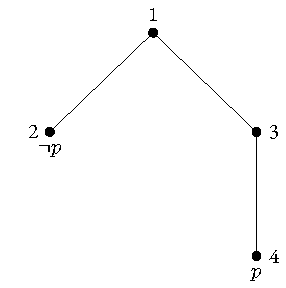
\includegraphics[width=0.8\linewidth,height=\textheight,keepaspectratio]{diagram.pdf}

}

\caption{\label{fig-kripke}A Kripke Tree to illustrate (P2)}

\end{figure}%

We introduce a ``weighting'' function \emph{w} by setting \emph{w}(1) =
0.2, \emph{w}(2) = 0.3, \emph{w}(3) = -0.1 and \emph{w}(4)~=~0.6. For
any \emph{A}, let \emph{P}(\emph{A})~=~\({\Sigma}\)\emph{w}(\emph{i}),
where the summation is across all points \emph{i} that force \emph{A}.
So \emph{P}(\emph{p})~= 0.6 and \emph{P}(\({\lnot}{\lnot}\)\emph{p}) =
0.5, contradicting (P2). But (P0), (P1), (P2′) and (P3) are all
satisfied, showing that (P2) is in the general case not derivable from
these three conditions.

\section{Bets and Intuitionistic Probability
Functions}\label{bets-and-intuitionistic-probability-functions}

Say that an \emph{A}-bet is a bet that pays \$1 if \emph{A} and nothing
otherwise. These will sometimes be called bets on \emph{A}. In this
theory, as in real life, it is possible that neither \emph{A}-bets nor
¬\emph{A}-bets will ever be collected, so holding an \emph{A}-bet and a
¬\emph{A}-bet is not necessarily as good as holding \$1. An \emph{A}-bet
becomes a winning bet, i.e.~worth \$1, just when it becomes known that
\emph{A}. We will assume that bookmakers and punters are both logically
proficient and honest, so that when a \emph{B}-bet becomes a winning bet
and \emph{B} \(\vdash_{IL}\) \emph{A}, then an \emph{A}-bet is a winning
bet. The picture underlying this story is the Kripke tree semantics for
intuitionistic logic. Bettors are thought of as being at some node of a
Kripke tree, an \emph{A}-bet wins at that stage iff \emph{A} is forced
by that node. Bettors do not know that any future nodes will be reached,
so they cannot be confident that all bets on classical tautologies
(\(\vdash_{CL}\)-theses) will be winning. And more importantly, we take
it that an (\emph{A}~∨~\emph{B})-bet wins if and only if an \emph{A}-bet
wins or a \emph{B}-bet wins. Again this mirrors the fact that
\emph{A}~∨~\emph{B} is forced at a node iff \emph{A} is forced or
\emph{B} is forced.

Finally, to get the Dutch Book style argument going, assume that for any
sequence of bets on \emph{A}\textsubscript{1},
\emph{A}\textsubscript{2}, \ldots, \emph{A}\textsubscript{\emph{k}}, the
bettor values the sequence at (\emph{Bel}(\emph{A}\textsubscript{1}) +
\emph{Bel}(\emph{A}\textsubscript{2}) + \ldots{} +
\emph{Bel}(\emph{A}\textsubscript{\emph{k}})). This is obviously
unrealistic and economically suspect\footnote{It is economically suspect
  because, in simplified terms, \emph{Bel}(\emph{A}) gives at best the
  use-value of an \emph{A}-bet, but this is distinct from the
  exchange-value the agent places on the bet. And it is the
  exchange-value that determines her patterns of buying and selling.},
but is perhaps a useful analogy. Then \emph{Bel} leads to coherent
valuations in all circumstances iff \emph{Bel} is a intuitionistic
probability function. That is, if \emph{Bel} is not an intuitionistic
probability function (henceforth: IPF) then there will be two finite
sequences of bets \emph{S}\textsubscript{1} and
\emph{S}\textsubscript{2} such that \emph{S}\textsubscript{1} is
guaranteed to pay at least as much as \emph{S}\textsubscript{2} in all
circumstances, but \emph{S}\textsubscript{2} is given higher value by
the agent. For simplicity \emph{Bel} will be called incoherent if this
happens, and coherent otherwise. If \emph{Bel} is an IPF there are no
two such sequences, so it is coherent.

If \emph{Bel} is not an IPF then we just need to look at which axiom is
breached in order to construct the sequences. For example, if (P3) is
breached then let the sequences be \(\langle\)\emph{A},
\emph{B}\(\rangle\) and \(\langle\)\emph{A}~∨~\emph{B},~\emph{A}
~∧~\emph{B}\(\rangle\). The same number of propositions from each
sequence are forced at every node of every Kripke tree, so the coherence
requirement is that the two sequences receive the same value. But
\emph{ex hypothesi} they do not, so \emph{Bel} is incoherent. Similar
proofs suffice for the remaining axioms (the remaining conditions on
\(\vdash\)-probability functions, that is, as they apply in the special
case of \(\vdash\) = \(\vdash_{IL}\)).

To show that if \emph{Bel} is an IPF it is coherent, we need some more
notation. Let \(\langle\)\emph{A}\textsubscript{1}, \ldots,
\emph{A}\textsubscript{\emph{k}}\(\rangle\) be a sequence of
propositions. Then say \emph{c\textsubscript{n}}\textsubscript{,}
\textsubscript{\emph{k}} is the proposition true iff at least \emph{n}
of these are true. So \emph{c}\textsubscript{2,3} is the proposition
(\emph{A}\textsubscript{1}~~∧~\emph{A}\textsubscript{2})~∨~(\emph{A}\textsubscript{1}~~∧~\emph{A}\textsubscript{3})~∨~(\emph{A}\textsubscript{2}~~∧~\emph{A}\textsubscript{3}).
Assuming \emph{Bel} is a IPF, we prove the following lemma holds for all
\emph{k}:

The proof is by induction on \emph{k}. For \emph{k}=1 and \emph{k}=2,
the proof is given by the axioms. So it remains only to complete the
inductive step. For ease of reading in the proof we write \emph{A} for
\emph{Bel}(\emph{A}) where no ambiguity would result.

By the inductive hypothesis we have:

\begin{figure*}

\begin{align*}
k\sum^{k+1}_{i=1}A_{i} &= k \sum^k_{i=1}c_{i,k} + kA_{k+1} \\
 &= (k-1)\sum_{i=1}^kc_{i,k} + \sum^k_{i=1}c_{i,k} + kA_{k+1} \\
 &= (k-1)\sum_{i=1}^{k}c_{i,k} + \sum^{k}_{i=1}(c_{i,k} \vee A_{k+1}) + (c_{i,k} \wedge A_{k+1}) \text{ by \textit{k} applications of (P3)}
\end{align*}

\end{figure*}%

Since
\(\sum_{i=1}^{k+1}A_i = \sum_{i=1}^{k}A_i + A_{k+1} = \sum_{i=1}^{k}c_{i,k} + A_{k+1}\),
this equation simplifies to:

\[
\sum_{i=1}^{k+1}A_i + (k-1)A_{k+1} = \sum_{i=1}{k}(c_{i,k} \vee A_{k+1}) + (c_{i,k} \wedge A_{k+1})
\]

Since \(c_{i,k} \vee A_{k+1}\) \(\dashv\)~\(\vdash\)
\(c_{i,k+1} \vee A_{k+1}\) and \(c_{i,k} \wedge A_{k+1}\)
\(\dashv\)~\(\vdash\) \(c_{i+1,k+1} \wedge A_{k+1}\) we have:

\[
\begin{aligned}
\sum_{i=1}^{k+1}A_i + (k-1)A_{k+1} &= \sum_{i=1}^{k}(c_{i,k+1} \vee A_{k+1}) + \sum_{i=1}^{k}(c_{i+1,k+1} \wedge A_{k+1})
\end{aligned}
\]

Now, \(c_{1,k+1} \vee~ A_{k+1}\) \(\dashv\)~\(\vdash\) \(c_{i,k+1}\) and
\(c_{k+1,k+1} ~\wedge~ A_{k+1}\) \(\dashv\)~\(\vdash\) \(c_{k+1,k+1}\)
from the definitions of \(c\). So substituting in these equivalences and
slightly renumbering, we get:

\[
\sum_{i=1}^{k+1}A_i + (k-1)A_{k+1} = c_{i,k+1} +c_{k+1,k+1} + \sum_{i=1}^{k-1}(c_{i+1,k+1} \vee A_{k+1}) + \sum_{i=1}^{k-1}(c_{i+1,k+1} \wedge A_{k+1})
\]

Regrouping the last two summations and applying (P3),

\begin{figure*}

\[
\begin{aligned}
\sum_{i=1}^{k+1}A_i + (k-1)A_{k+1} &= c_{1,k+1} + c_{k+1,k+1} + \sum_{i=1}^{k-1}c_{i+1,k+1} + A_{k+1} \\
&= \sum_{i=1}^{k+1}c_{i+1,k+1} + (k-1)A_{k+1}
\end{aligned}
\]

\end{figure*}%

And cancelling out the second term on each side gives us the result we
want. From this it follows immediately that \emph{Bel} is coherent. Let
\emph{S}\textsubscript{1} and \emph{S}\textsubscript{2} be any two
sequences such that \emph{S}\textsubscript{1} is guaranteed to pay as
much as \emph{S}\textsubscript{2}. That is, that
\emph{S}\textsubscript{2} pays \$\emph{n} entails
\emph{S}\textsubscript{1} pays at least \$\emph{n} for all \emph{n}. Now
the lemma shows that for each sequence of bets, their value equals the
sum of the probability that they'll pay at least \emph{n} for all values
of \emph{n}, up to the length of the sequence. So by as many appeals to
(P2) as there are bets in \emph{S}\textsubscript{1}, we have that the
value of \emph{S}\textsubscript{2} is less than or equal to the value of
\emph{S}\textsubscript{1}, as required.

Given the well-known problems with Dutch Book arguments\footnote{See
  Maher (\citeproc{ref-Maher1993}{1993}) for criticisms of the most
  recent attempts at successful Dutch Book arguments and references to
  criticisms of earlier attempts.}, it might be wondered if we can give
a different justification for the axioms. Indeed it may be considered
helpful to have a semantics for the logic which does not refer to
betting practices. One possibility is to say that IPFs are normalised
measures on Kripke trees. The idea is that the probability of a
proposition is the measure of the set of points at which the proposition
is forced. It is straightforward to give a non-constructive proof that
the axioms are sound with respect to these semantics, but making this
proof constructive and providing any proof that the axioms are complete
is a harder task. So for now this Dutch Book justification for the
axioms is the best available.

\section*{Appendix: The Morgan--Leblanc--Mares
Calculus}\label{appendix-the-morganleblancmares-calculus}
\addcontentsline{toc}{section}{Appendix: The Morgan--Leblanc--Mares
Calculus}

In a series of papers ((\citeproc{ref-MorganLeBlanc1983a}{Morgan and
LeBlanc 1983a}, \citeproc{ref-MorganLeBlanc1983b}{1983b}), Morgan and
Mares (\citeproc{ref-MorganMares1995}{1995})) an approach to probability
grounded in intuitionistic logic has been developed. The motivation is
as follows. A machine contains an unknown set of propositions \emph{S},
which need not be consistent. \emph{Pr}(\emph{A}, \emph{B}) is the
maximal price we'd pay for a bet that \emph{S} and \emph{B}
intuitionistically entail \emph{A} (\emph{S},~\emph{A} \(\vdash_{IL}\)
\emph{B}, that is). By standard Dutch Book arguments, we obtain axioms
for a probability calculus which has some claim to being constructivist.
The point of this section is to register the shortcomings of this
approach as a theory of uncertain reasoning from evidence -- to point
out, that is, the implausibility of interpreting the axioms they derive
as normative constraints on degrees of belief. (It should be noted from
the start that this was \emph{not} the advertised purpose of their
theory, and at least one of the authors (Mares) has said (p.c.) that the
primary purpose of constructing these theories was to generalise of the
triviality results proved in Lewis (\citeproc{ref-Lewis1976b}{1976}). So
the purpose of this appendix may be to argue for something that isn't in
dispute: that these theories can't be pushed into double duty as
theories of reasoning under uncertainty.)

The axiomatisations given in the Morgan and Leblanc papers differs a
little from that given in the Morgan and Mares paper, but the criticisms
levelled here apply to their common elements. In particular, the
following four axioms are in both sets.

\begin{description}
\tightlist
\item[(C1)]
0 \({\leq}\) \emph{Pr}(\emph{A}, \emph{B})~\({\leq}\)~1
\item[(C2)]
\emph{Pr}(\emph{A}, \emph{A}~~∧~\emph{B}) = 1
\item[(C3)]
\emph{Pr}(\emph{A}, \emph{B}~~∧~\emph{C})~ \emph{Pr}(\emph{B}, \emph{C})
= \emph{Pr}(\emph{B}, \emph{A}~~∧~\emph{C})~ \emph{Pr}(\emph{A},
\emph{C})
\item[(C4)]
\emph{Pr}(\emph{A}~\({\supset}\)~\emph{B}, \emph{C}) =
\emph{Pr}(\emph{B}, \emph{A}~~∧~\emph{C})
\end{description}

These four are enough to get both the unwanted consequences. In
particular, from these we get the `no negative evidence' rule:
\emph{Pr}(\emph{A}, \emph{B}~~∧~\emph{C})~\({\geq}\) \emph{Pr}(\emph{A},
\emph{B}). The proof is in Morgan and Mares
(\citeproc{ref-MorganMares1995}{1995}) Now given the semantic
interpretation they have adopted, this is perhaps not so bad. After all,
if we can prove \emph{A} from \emph{B} and \emph{S}, we can certainly
prove it from \emph{B}~~∧~\emph{C} and \emph{S}, but the converse does
not hold. However from our perspective this feature seems a little
implausible. In particular, if \emph{C} is ¬\emph{A}, it seems we should
have \emph{Pr}(\emph{A}, \emph{B}~~∧~¬\emph{A}) = 0 unless
\emph{B}~\(\vdash_{IL}\)~\emph{A}, in which case
\emph{Pr}(\emph{A},~\emph{B}~~∧~¬\emph{A}) is undefined.

It shouldn't be that surprising that we get odd results given (C4).
Lewis (\citeproc{ref-Lewis1976b}{1976}) shows that adopting it for a
(primitive or defined) connective `\({\rightarrow}\)' within the
classical probability calculus leads to triviality. And neither the
arguments he uses there nor the arguments for some stronger conclusions
in Lewis (\citeproc{ref-Lewis1999b}{1999}) rely heavily on classical
principles. The papers by Morgan and Leblanc don't discuss this threat,
but it is taken discussed in detail in Morgan and Mares
(\citeproc{ref-MorganMares1995}{1995}). Morgan and Mares note that it's
possible to build a theory based on (C1) to (C4) that isn't trivial in
the sense Lewis described. But these theories still have enough
surprising features that they aren't suitable for use as a theory of
reasoning under uncertainty.

In intuitionistic logic we often take the falsum \({\perp}\) as a
primitive connective, functioning as a \(\vdash_{IL}\)-antithesis. Hence
a set \emph{S} is intuitionistically consistent iff we do not have
\emph{S} \(\vdash_{IL}\) \({\perp}\). Now the following seems a
plausible condition:

\begin{description}
\item[(C\({\perp}\))]
For consistent \emph{B}, \emph{Pr}(\({\perp}\), \emph{B}) = 0.
\end{description}

Given consistent evidence, we have no evidence at all that the falsum is
true. Hence we should set the probability of the falsum to 0 (as
required by our condition (P0) from Section 1). Given Morgan and
Leblanc's original semantic interpretation there is less motivation for
adopting (C\({\perp}\)), since \emph{S} might be inconsistent. The
restriction to consistent \emph{B} in (C\({\perp}\)) is imposed because
we take \emph{Pr}(\emph{A}, \emph{B}) to be undefined for inconsistent
\emph{B}, as explained at the end of Section 1. (In more detail: if
\emph{B} is a \(\vdash_{IL}\)-antithesis then \emph{Pr}(\emph{B}) = 0
for any intuitionistic probability function \emph{Pr}, whence the
undefinedness of \emph{Pr}(\emph{A}, \emph{B}) by the remarks at the end
of that section.) Morgan, Leblanc and Mares take it to be set at 1. The
choice here is a little arbitrary, the only decisive factor being
apparently the easier statement of certain results. Now if we take the
falsum as a primitive the next move is usually to introduce ¬ as a
defined connective, as follows.

¬\emph{A}~=\textsubscript{df} \emph{A}~\({\supset}\)~\({\perp}\)

Assuming \emph{A}~~∧~\emph{B} is consistent, it follows from (C4) and
(C\({\perp}\)) that \emph{Pr}( ¬\emph{A}, \emph{B}) = 0. Again, from our
perspective this is an implausible result. The main purpose of this
appendix has been to show that the Morgan--Leblanc--Mares probability
calculus cannot do the work Bayesians want a probability calculus to do.
That is, it is implausible to regard their \emph{Pr}(\emph{A}, \emph{B})
as the reasonable degree of belief in \emph{A} given \emph{B}. Hence the
account of conditional probability these authors offer diverges from the
intuitionistic Bayesianism that we have been urging heterodox theorists
to endorse.\footnote{Thanks to Alan Hájek, Graham Oppy and, especially,
  Lloyd Humberstone for comments and suggestions on various drafts of
  this paper.}

\subsection*{References}\label{references}
\addcontentsline{toc}{subsection}{References}

\phantomsection\label{refs}
\begin{CSLReferences}{1}{0}
\bibitem[\citeproctext]{ref-Christensen1996}
Christensen, David. 1996. {``Dutch-Book Arguments {D}e-Pragmatized:
Epistemic Consistency for Partial Believers.''} \emph{Journal of
Philosophy} 93 (9): 450--79. doi:
\href{https://doi.org/10.2307/2940893}{10.2307/2940893}.

\bibitem[\citeproctext]{ref-Cohen1977}
Cohen, L. Jonathan. 1977. \emph{The Probable and the Provable}. Oxford:
Clarendon Press.

\bibitem[\citeproctext]{ref-Dempster1967}
Dempster, Arthur. 1967. {``Upper and Lower Probabilities Induced by a
Multi-Valued Mapping.''} \emph{Annals of Mathematical Statistics} 38:
325--39. doi:
\href{https://doi.org/10.1214/aoms/1177698950}{10.1214/aoms/1177698950}.

\bibitem[\citeproctext]{ref-Harman1983}
Harman, Gilbert. 1983. {``Problems with Probabilistic Semantics.''} In
\emph{Developments in Semantics}, edited by Alex Orenstein and Rafael
Stern, 243--37. New York: Haven.

\bibitem[\citeproctext]{ref-Hellman1997}
Hellman, Geoffery. 1997. {``Bayes and Beyond.''} \emph{Philosophy of
Science} 64 (2): 191--221. doi:
\href{https://doi.org/10.1086/392548}{10.1086/392548}.

\bibitem[\citeproctext]{ref-HowsonUrbach1989}
Howson, Colin, and Peter Urbach. 1989. \emph{Scientific Reasoning}. La
Salle: Open Court.

\bibitem[\citeproctext]{ref-Joyce1998}
Joyce, James M. 1998. {``A Non-Pragmatic Vindication of Probabilism.''}
\emph{Philosophy of Science} 65 (4): 575--603. doi:
\href{https://doi.org/10.1086/392661}{10.1086/392661}.

\bibitem[\citeproctext]{ref-Kaplan1996}
Kaplan, Mark. 1996. \emph{Decision Theory as Philosophy}. Cambridge:
Cambridge University Press.

\bibitem[\citeproctext]{ref-Lewis1976b}
Lewis, David. 1976. {``Probabilities of Conditionals and Conditional
Probabilities.''} \emph{Philosophical Review} 85 (3): 297--315. doi:
\href{https://doi.org/10.2307/2184045}{10.2307/2184045}. Reprinted in
his \emph{Philosophical Papers}, Volume 2, Oxford: Oxford University
Press, 1986, 133-152. References to reprint.

\bibitem[\citeproctext]{ref-Lewis1999b}
---------. 1999. {``Why Conditionalize?''} In \emph{Papers in
Metaphysics and Epistemology}, 403--7. Cambridge University Press.
Originally written as a course handout in 1972.

\bibitem[\citeproctext]{ref-Maher1993}
Maher, Patrick. 1993. \emph{Betting on Theories}. Cambridge: Cambridge
University Press.

\bibitem[\citeproctext]{ref-MorganLeBlanc1983a}
Morgan, Charles, and Hughes LeBlanc. 1983a. {``Probabilistic Semantics
for Intuitionistic Logic.''} \emph{Notre Dame Journal of Formal Logic}
24 (2): 161--80. doi:
\href{https://doi.org/10.1305/ndjfl/1093870307}{10.1305/ndjfl/1093870307}.

\bibitem[\citeproctext]{ref-MorganLeBlanc1983b}
---------. 1983b. {``Probability Theory, Intuitionism, Semantics and the
Dutch Book Argument.''} \emph{Notre Dame Journal of Formal Logic} 24
(3): 289--304. doi:
\href{https://doi.org/10.1305/ndjfl/1093870372}{10.1305/ndjfl/1093870372}.

\bibitem[\citeproctext]{ref-MorganMares1995}
Morgan, Charles, and Edward Mares. 1995. {``Conditionals, Probability
and Non-Triviality.''} \emph{Journal of Philosophical Logic} 24 (5):
455--67. doi:
\href{https://doi.org/10.1007/bf01052599}{10.1007/bf01052599}.

\bibitem[\citeproctext]{ref-Paris1994}
Paris, J. B. 1994. \emph{The Uncertain Reasoner's Companion: A
Mathematical Perspective}. Cambridge: Cambridge University Press.

\bibitem[\citeproctext]{ref-Ponsonnet1996}
Ponsonnet, Jean-Marc. 1996. {``The Best and the Worst in g. L. S.
Shackle's Decision Theory.''} In \emph{Uncertainty in Economic Thought},
edited by Christian Schmidt, 169--96. Cheltham: Edward Elgar.

\bibitem[\citeproctext]{ref-RamseyTruthProb}
Ramsey, Frank. 1926. {``Truth and Probability.''} In \emph{Philosophical
Papers}, edited by D. H. Mellor, 52--94. Cambridge: Cambridge University
Press.

\bibitem[\citeproctext]{ref-Savage1954}
Savage, Leonard. 1954. \emph{The Foundations of Statistics}. New York:
John Wiley.

\bibitem[\citeproctext]{ref-Schmeidler1989}
Schmeidler, David. 1989. {``Subjective Probability and Expected Utility
Without Additivity.''} \emph{Econometrica} 57 (3): 571--89. doi:
\href{https://doi.org/10.2307/1911053}{10.2307/1911053}.

\bibitem[\citeproctext]{ref-Shackle1949}
Shackle, George. 1949. \emph{Expectation in Economics}. Cambridge:
Cambridge University Press.

\bibitem[\citeproctext]{ref-Shafer1976}
Shafer, Glenn. 1976. \emph{A Mathematical Theory of Evidence}.
Princeton: Princeton University Press.

\bibitem[\citeproctext]{ref-Shafer1981}
---------. 1981. {``Constructive Probability.''} \emph{Synthese} 48 (1):
1--60. doi:
\href{https://doi.org/10.1007/bf01064627}{10.1007/bf01064627}.

\bibitem[\citeproctext]{ref-Teller1973}
Teller, Paul. 1973. {``Conditionalization and Observation.''}
\emph{Synthese} 26 (2): 218--58. doi:
\href{https://doi.org/10.1007/bf00873264}{10.1007/bf00873264}.

\bibitem[\citeproctext]{ref-Zadeh1978}
Zadeh, Lofti A. 1978. {``Fuzzy Sets as a Basis for a Theory of
Probability.''} \emph{Fuzzy Sets and Systems} 1 (1): 3--28. doi:
\href{https://doi.org/10.1016/0165-0114(78)90029-5}{10.1016/0165-0114(78)90029-5}.

\end{CSLReferences}



\noindent Published in\emph{
Notre Dame Journal of Philosophical Logic}, 2001, pp. 111-123.


\end{document}
